\subsection{Preparing to return}

\section{"The Thirst to be First"}

Want to bag an unclimbed peak? Fine. Check it out on googlemaps; blow your student loan on a long distance flight and take your chances with the weather and with the fate of your Sherpas. You can phone your mum from the top.

\margininbox{Slov trig Points}{Hi, Jarvist

On internet, (http://kremen.arso.gov.si/ NVatlas- but you need registration) I find GK coordinates of Trig Points:

\begin{itemize}
    \item352 Tolminski Migovec: 5405022,6 5123150,0
    \item20 Vrh nad Skrbino: 5406302,7 5124087,4
    \item364 Grusnica: 5403984,6 5122439,8
    \item120 Planina Razor: 5407087,3 5122035,1
    \item55 Tolminski Kuk: 5404539,7 5124804,8 
    \end{itemize}
\protect\mininame{Via Zdenko, 2006}}{\logbook}



Caving exploration is not like this. There is only one way of discovering what lies beneath, and that is to go there. We don't just venture to extreme places, but survey and map and bolt and hammer. We start not with satellite data and 1:10'000 scale maps, but with a simple blank sheet.

And when underground -- there is just you and your friends. There is no radio that can penetrate through half a kilometer of solid rock. No helicopter rescues, no satellite phone. Utter self-reliance and cooperation begin on day one, and go on to form extremely strong relationships.

We don't just go there -- we bring these places into being by our perseverance and hard work, smoothing the way and spreading the word so that the next team, whether in 2010 or 2100 can take up the baton in this never ending relay race to unlock the very secrets of the Earth.

\name{Jarvist Frost}



Every year Imperial College Caving Club recruits new cavers -- and happily, by the end of the academic year, there has always been at least one newbie interested in exploring \passage{Migovec}. A description like the above might have convinced an undergraduate to try out caving the October before.

For every year that the expedition goes to Migovec, there is of course also an accompanying round of funding applications. After a year away from Slovenia in 2006, spirits were high for the 2007 expedition. The following report for the Imperial College Exploration Board provides both a summary of those hopes, and a counterpoint most interesting. We can now look over these aims and ideas with the benefit of hindsight, but at the time, who could know what was to come?

\name{Fiona Hartley}

\newpage

\subsection{Migovec Explorations 2007}
\textit{A request for funding from the Imperial College Exploration Board, dated January 2007}

\subsection{Abstract}

Over the last twelve years, students from Imperial College Caving Club have been exploring cave systems beneath \passage[mountain]{Tolminski Migovec} in western Slovenia. Working in full cooperation with the local club (JSPDT), we have discovered over 20 km of cave passage, going down to a depth (-970 m) of twice the maximum attainable in the UK.

We are in an extremely privileged position to explore this mountain with such autonomy. No other alien caving group can explore Slovenian caves in this fashion. Being one of the few elite student groups who explore new caves in extremely deep and cold alpine systems brings Imperial considerable kudos from international speleological circles.


\begin{pagefigure}
      \checkoddpage \ifoddpage \forcerectofloat \else \forceversofloat \fi
      \centering
              \frame{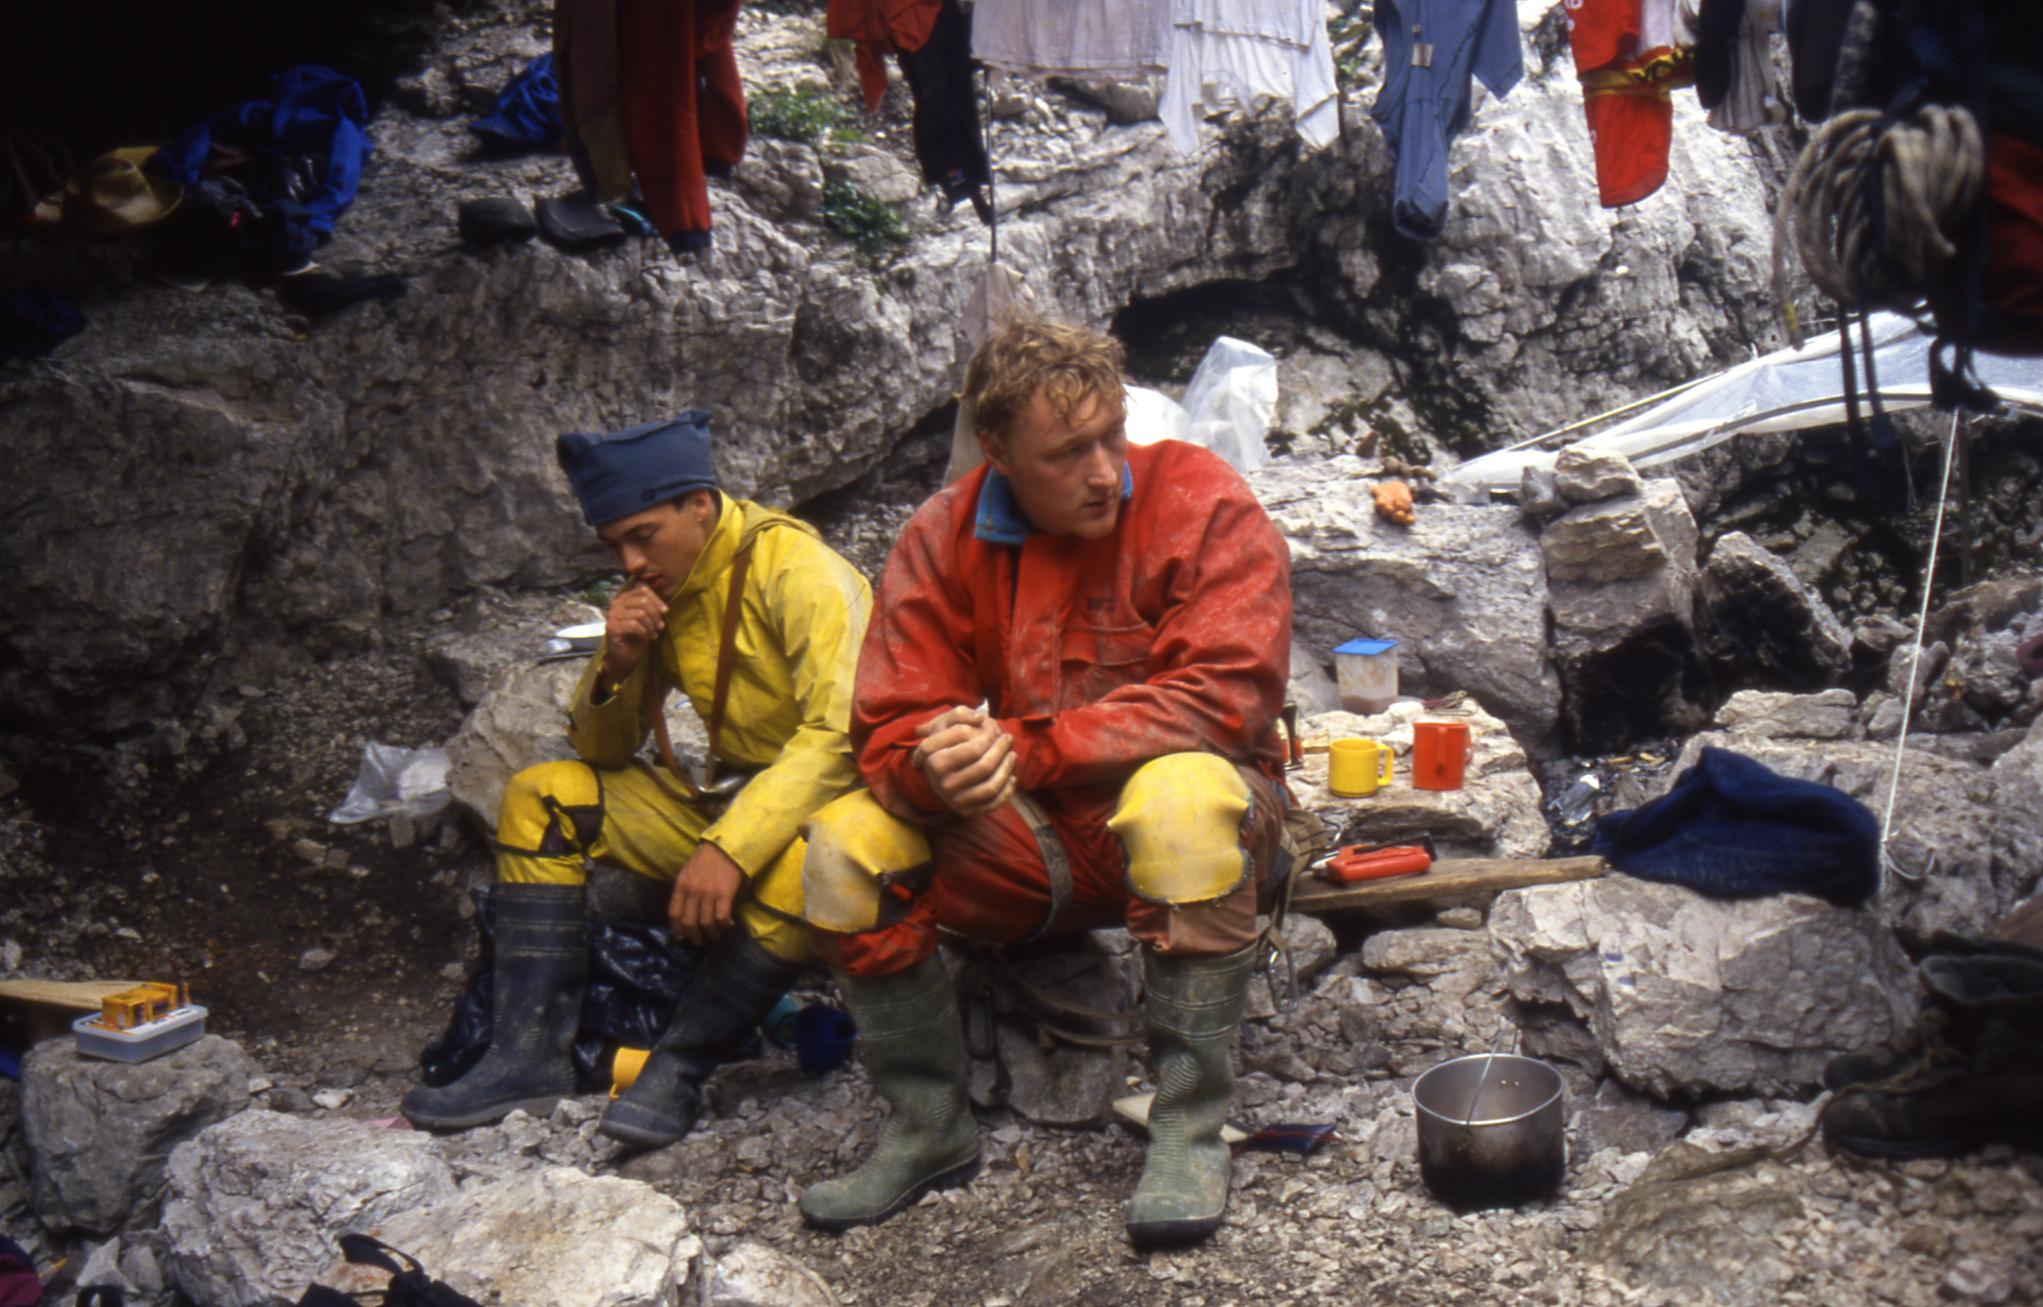
\includegraphics[width=\linewidth]{2007/exploboard2007/1994-iain mckenna-jim and andy--orig.jpg}} 
       \label{surface bashing}
  \caption{ICCC has been exploring the caves beneath \passage[mountain]{Tolminski Migovec} from the \passage{Bivi} since 1994. \pic{Iain McKenna}}
\end{pagefigure}


We do not just explore, but make accurate survey measurements, publish detailed drawn surveys of the caves and coordinate with local research scientists to carry out hydrological and geomorphic studies as well as biological surveys and sample collection. \passage[mountain]{Migovec} is located on the major \passage{Bovec fault}, and stands on the watershed of the Adriatic and Black seas -- making it of extreme interest and the focus of international research.

\marginnote{The Hollow Mountain 1974-2006 would be published in late 2007.}

We are in the process of publishing a full bound report of our activities from 1994-2006, which as a standalone report we fully expect to have worldwide distribution with an initial print-run of 200 copies. Our explorations this year will be presented at the national caving conference in September, via our website and through bulletins submitted to 'Descent' and the British Cave Research Association.

\marginnote{Descent is a British and Irish bimonthly caving magazine, first issued in 1969. Chris Howes and Judith Calford  edited the magazine during the period covered in this journal.}

From the prospective of our club, the \passage[mountain]{Migovec} explorations have been the lynch pin keeping us at the very height of our sport, and ensuring a continuity of skills transfer between members. As usual, the prospective expedition members cover an enormous range of ages and experience -- from our 1986 President to first years.

The \passage[mountain]{Migovec} plateau has three main caves, all of which are under one-hundred metres at close approach. The interconnection of these into \passage{Sistem Migovec} would almost certainly result in the largest system in Slovenia. Already the cave is extremely complex at great depth, in a fashion that has not be observed in any other high-altitude alpine system. Though by having concentrated tens of man-years of effort into exploring one tiny area we have sacrificed our rate of passage discovery (expecting a 'mere' kilometre or two per year), we have gained a far more comprehensive and complete understanding.

The expedition nature of this operation cannot be overstressed. From start to finish it is motivated by the true spirit of exploration. Commitment from members in terms of time, arduous undertakings and endurance are unparalleled in our day-to-day operation of the club. We are a comparatively cheap expedition. This is due to our knowledge of the situation, our local contacts (arranging special permission to camp gratis in the national park, safe free parking of the minibus, free safe storage of our gear in the barn at \passage[town]{Ravne}, etc.), our year-on-year investment in this project and general efficiency.

\bignote{After a 'year out' having not gone on expedition in 2006, there is a great hunger for the genuine exploration that will be on offer this summer}. I am sure that this year will be an extremely productive one on the \passage[mountain]{Migvoec} Plateau.


\subsection{Aims}

Thanks to light-weight recce work done by this club in October 2005 \& Autumn 2006, as well as exploration done by the JSPDT, an enormous number of leads are currently in the process of being explored.


\subsection{Deep Exploration in Vrtnarija / Gardeners' World}

The steel self-driving bolts that we use to secure our ropes rust. The rate of decay can make them unsafe to use in anywhere between just a couple of years and a decade (depending on humidity and temperature). Similarly, our ropes are left in place in the caves (coiled above the pitches in a dry location) and will also decay over the years. \passage{Vrtnarija}, a cave discovered in 2000, has a number of leads distributed throughout its length. The re-rigging of this cave from step would would represent such a large financial, logistical and man-power effort that is unlikely to happen considering the far easier leads elsewhere.

As such, this is liable to be the last year in which 'deep' exploration will occur.

There is a large walking passage at -800 which was left unexplored in 2004 due to lack of time.

\begin{marginfigure}
\frame{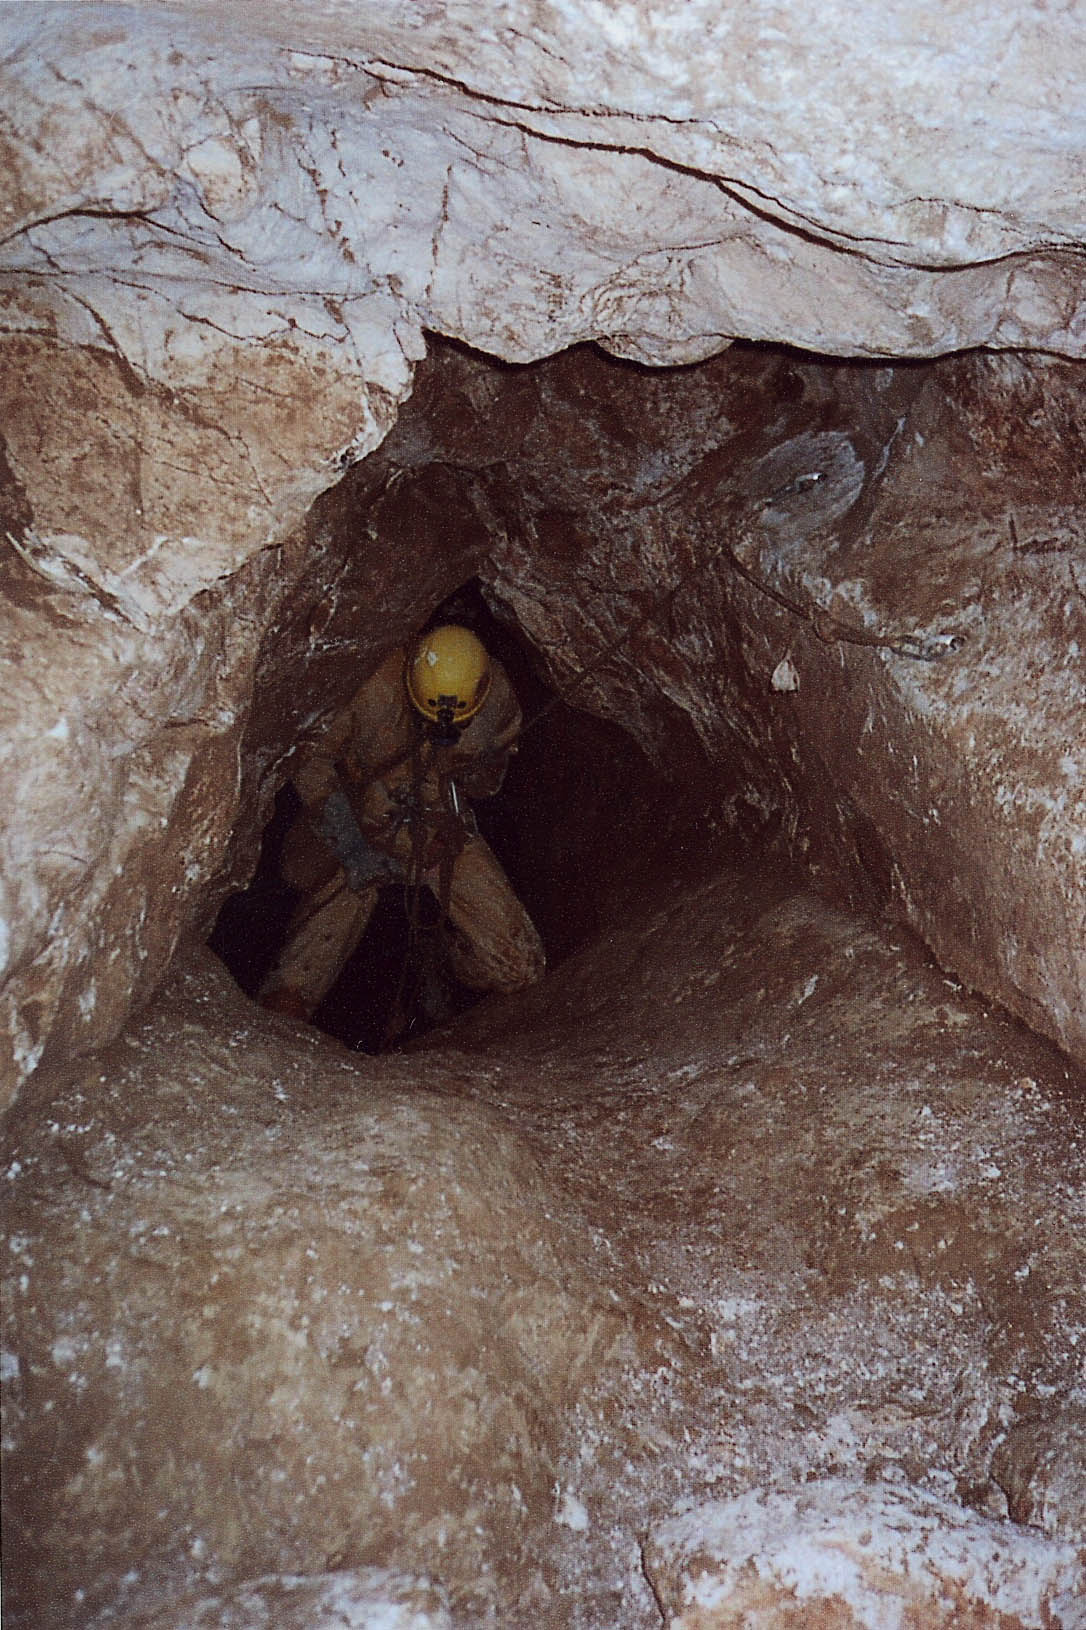
\includegraphics[width=\linewidth]{2007/exploboard2007/2004-aps-evetts15-MartinTopOfBigRockCandyMountain--orig.jpg}}
\caption{The top of \passage{Big Rock Candy Mountain} in 2004. \pic{Jan Evetts}}
\end{marginfigure}

The sump (\passage{Colorado}) consists of an aven which should be aid-climbed to find out whether it is merely a perched sump or is in fact the  termination of the cave (this is a matter of considerable scientific interest, as the location of such sumps within the \passage[mountain]{Migovec} plateau serve as an indicator to the shape and slope of the impermeable shale layer upon which the limestone massif rests).

Slightly further back from \passage{Colorado} there is a large aven ('\passage{To Infinity and Beyond}') which should be climbed to ascertain whether it breaks into a separate cave system. This part of the cave is nearly 2km horizontally from the entrance, underneath one of the mountain peaks ('\passage[mountain]{Kuk}') which form the 'crown' of the plateau. It is quite possible that a different cave descends from a lower-level plateau north of \passage[mountain]{Kuk} and drains into the Adriatic catchment. This is of obvious interest in terms of understanding the hydrology of the watershed.

Again, in the very low level ($\approx$ -800 m), another such aven ('\passage{Strap on the Nitro}, Aven') indicates a connection to another cave system. This aven is almost directly below the termination of '\passage{Exhibition Road}' in \passage{SysMig}.

Higher up in \passage{Vrtnarija}, there are windows that have been noticed across from the top of pitch-heads. These will require a bolt-traverse to reach, but again offer the possibility of connection into otherwise isolated sections of the cave. In particular, the top of '\passage{Big Rock Candy Mountain}' and '\passage{Zimmer}' (-500 m) will require serious attention, as will the tunnel noticed above '\passage{Laurel}'.
Our 2005 expedition concentrated on pushing a window leading off from '\passage{Pico}', which is believed to connect back into '\passage{Space Odyssey}'. A confirmation of this connection, exploration of the \passage{Space Odyssey} aven and exploration of a perched mud sump ('\passage[sump]{Mud Slump}') will also be targets.

To explore these areas in a safe \& efficient manner, an underground camp will be necessary. Our likely camping spot is 'Camp \passage{X-Ray}', the location of the 2003 camp at -600 m. Deep exploration parties will descend in one day, sleep, explore the limit of exploration before returning to camp, sleep, and then spend a day exiting the cave.

The costs for non-personal caving gear this year are considerable. Aid-climbing equipment is necessary (lightweight battery operated drill, sufficiently large solar charging system, dynamic ropes, many disposable rock anchors), and the descent to -800 m will require piecemeal replacements made to the rigging equipment.

\subsection{Primadona}

In Oct 2006, a lightweight JSPDT/ICCC exploration trip went to -300m in \passage{Primadona} (a cave system on the western flank of the plateau) in order to explore the region '\passage{Smer0}' closest to \passage{System Migovec}. This area of the cave is extremely interesting, wherein the rock change from a dirty shattered limestone that typifies \passage{Primadona} to the smooth soft pure-white limestone that was noticeable almost throughout \passage{SysMig}. As well as discovering a higher-level passage that reconnected in the rift, an active stream was discovered that crossed the fossilised passage. This stream, flowing East-West is approximately one hundred metres from the '\passage{XXX}' pitch in \passage{SysMig}, where a river enters as a waterfall. A connection is most eagerly anticipated.

\margininbox{Keyhole / Postcard}{

\passage{Keyhole Cave} and \passage{Postcard Cave} are very near the bivvy. The easiest way to describe them is to start from the edge of the shakehole with \passage{Hare Cave} in. Facing towards \passage{primadoni} direction \passage{Hare Cave} is on the left side of the shake hole. Basically you are standing above \passage{Postcard Cave}. It is in a smaller shakehole behind you. The entrance is a very low thin bedding plane that immediately breaks into an 'impressive' entrance phreatic tube with a choked draughting rift in the floor. This looks like many other entrances, so the way to confirm is that \passage{Keyhole Cave} should also be present in the shakehole. Still facing the same way (i.e. away from the shakehole towards the \passage{Hare Cave} shakehole), \passage{Keyhole Cave} is on the left side and is almost completely invisible unless you are standing in exactly the right place. Entrance is a lovely phreatic keyhole about 1m high and really very hidden. The cave follows this shape for a couple of metres before ending in a choked small chamber. Not that interesting but a great entrance - would make a superb start to a trip.

\protect\mininame{Ben Ogborne, Written Spring 2007, remembered from 2004 expo}}{\logbook}


\subsection{Razor / Moth / Hare / Keyhole / Postcard / Storm / K9 / K2 / K12 \& others}

As ever, we are exploring the plateau with an eye not just to next year, but to the next decade. A number of small surface caves are in active exploration, and we will most certainly be performing more surface exploration, documentation and mapping over the summer. These allow us to train novice cavers in the many specialised techniques and skills necessary for exploration in a safe environment, as well as being able to encourage a 'hunger for exploration' in having your own cave to push and explore.

\subsection{Hawk Cave}

Rediscovered in October 2006, after having been lost for nearly 30 years, an initial exploratory trip was made in adverse weather conditions. Situated on the western edge of the plateau, above the complex of \passage{Primadona} yet protected from filling with debris by an overhanging cliff, \passage{Hawk Cave} has enormous potential. Passages continue on many levels, and it will be immediately pushable by first-year cavers.

\begin{figure*}[t!]
\checkoddpage \ifoddpage \forcerectofloat \else \forceversofloat \fi
\frame{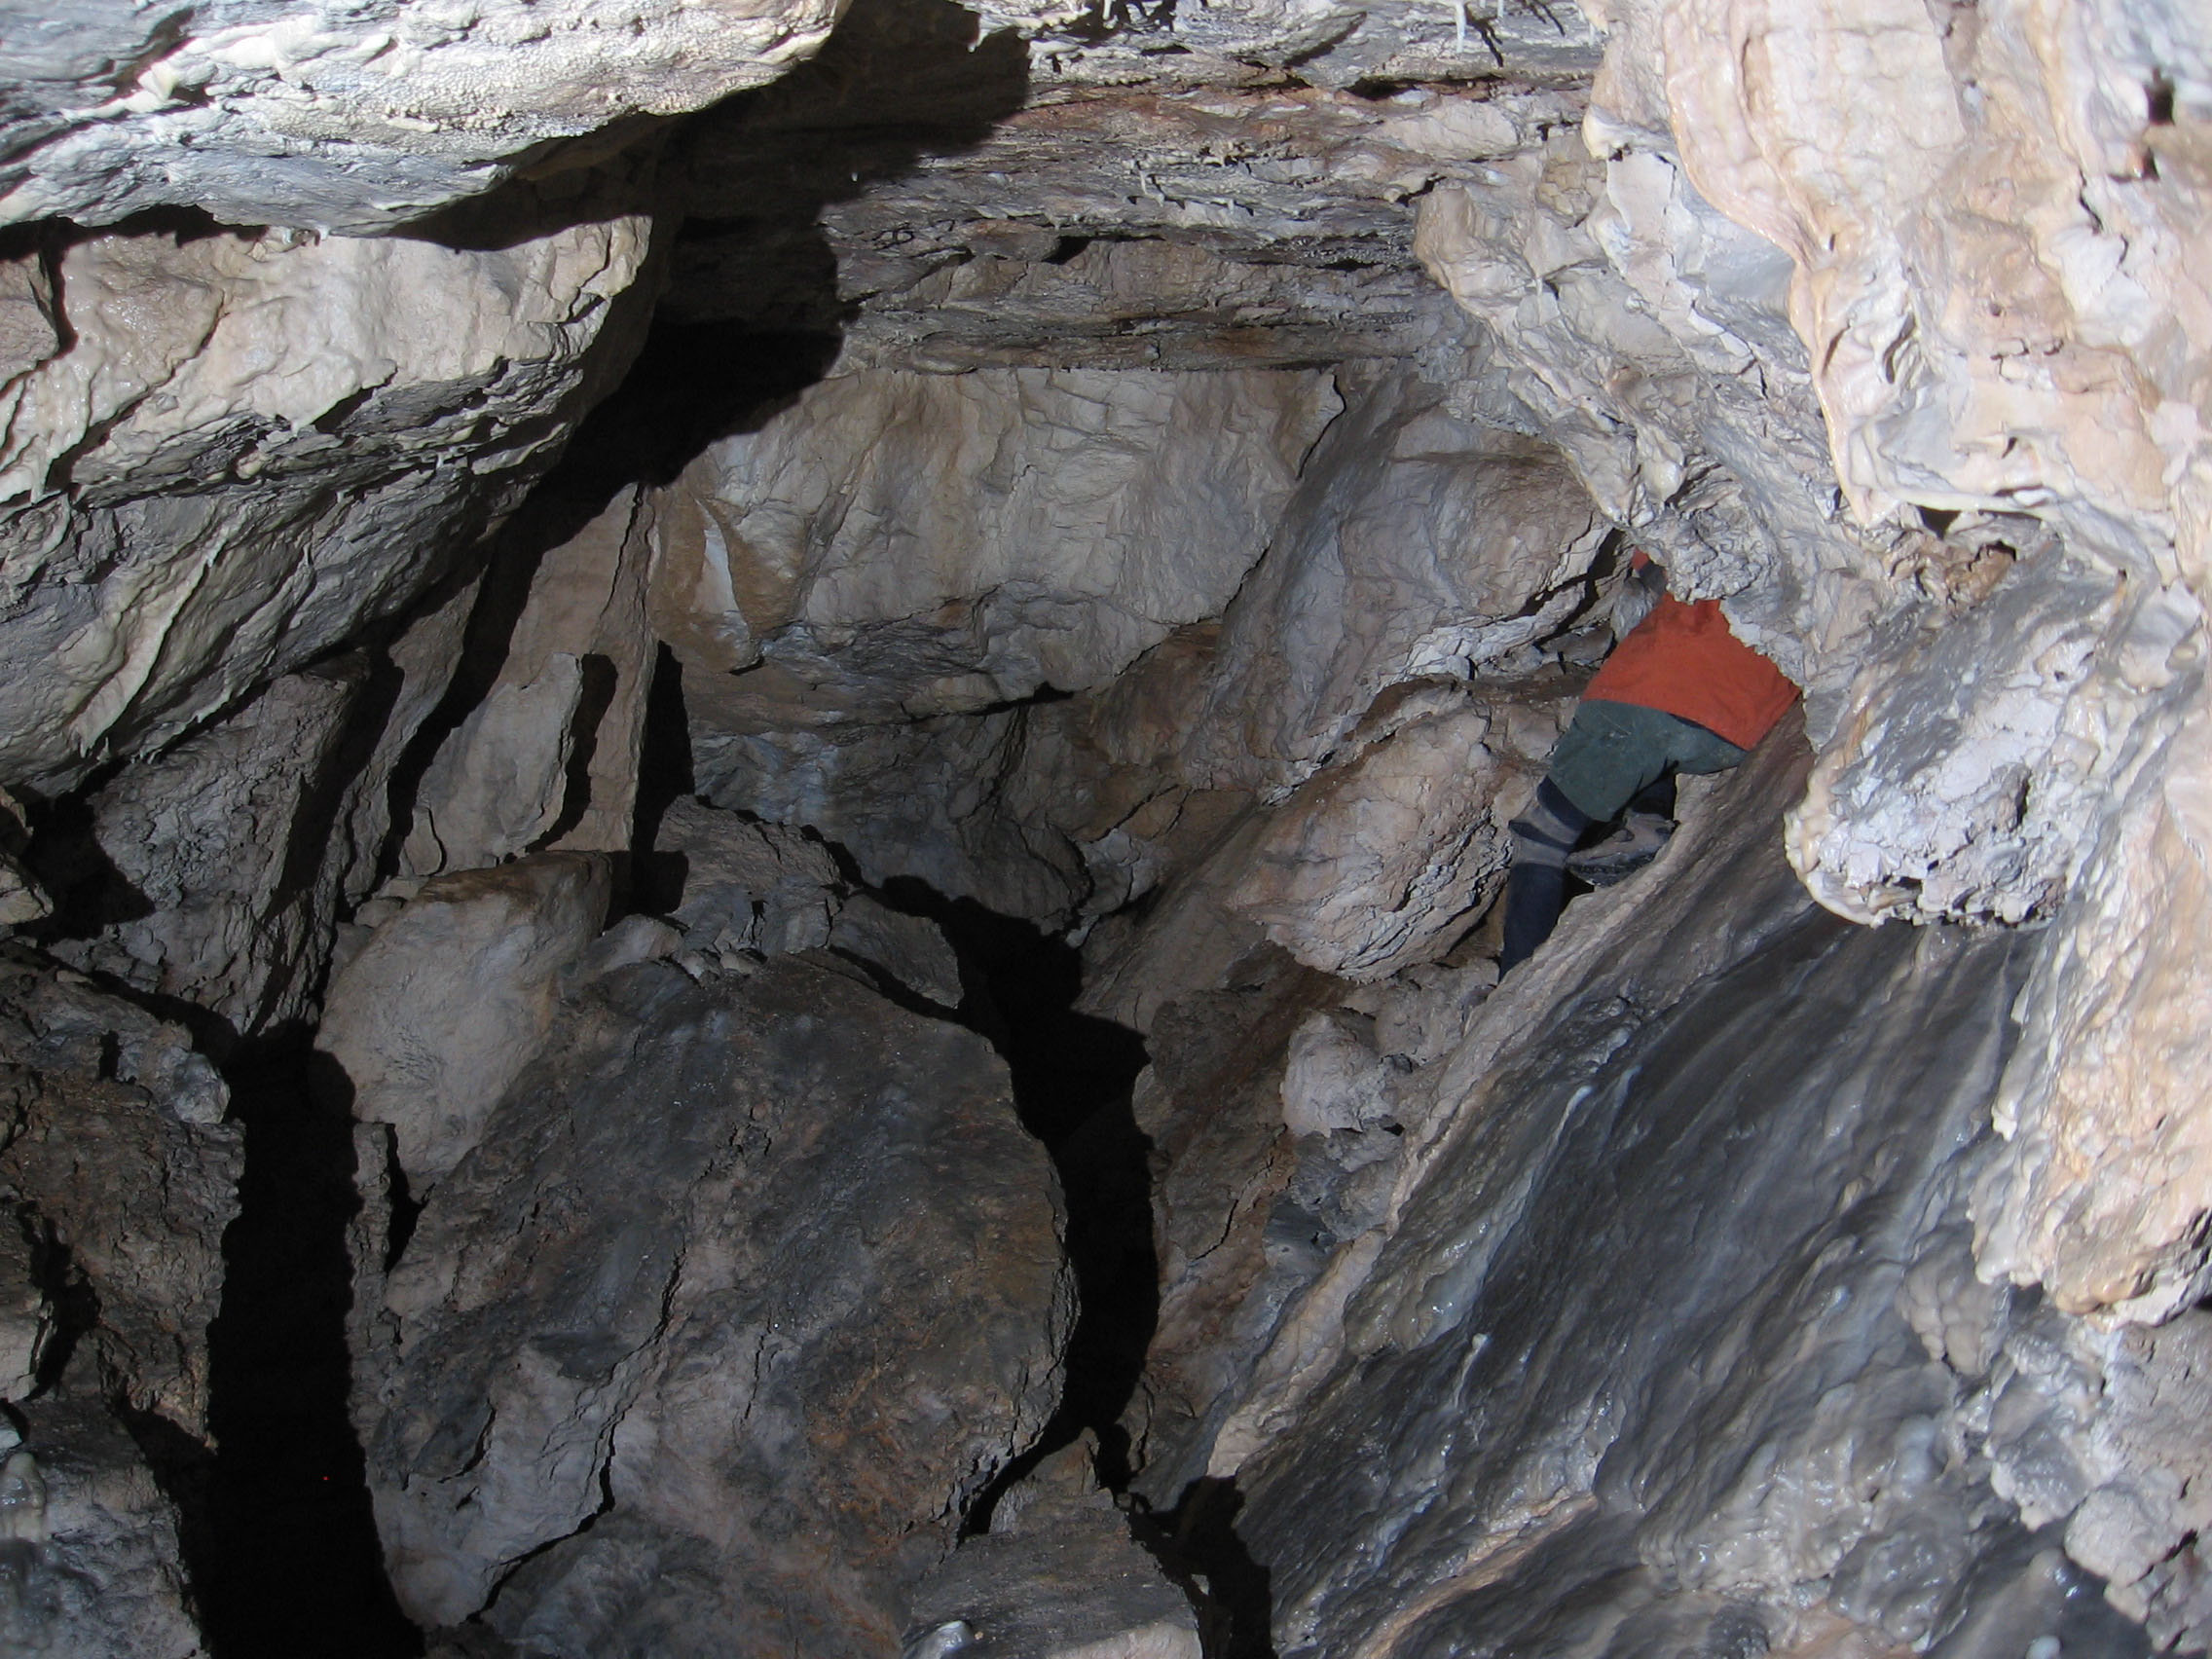
\includegraphics[width=\linewidth]{2007/exploboard2007/2006-Razor Cave-Lead in Second Chamber--orig.jpg}}
\caption{Tetley in \protect\passage{Razor Cave}, a prospect for further exploration in 2007. \pic{Jarvist Frost}}
\end{figure*}

\subsection{Logistics}

The majority of the food shopping is done in bulk a week before the expedition. High altitude food does not have to be expensive - you will not find dehydrated icecream or ration packs amongst our provisions. Due to lack of refrigeration, the food is vegetarian - except for the canned fish taken to underground camp. Menus are carefully balanced to ensure protein completeness, with most meals being built around a legume core (lentils, kidney beans, TVP\sidenote{Textured Vegetable Protein, infamous for causing flatulence}) with a variety of dried vegetables. Hard chedder cheese is bought in bulk and found to keep for the duration of the expedition if stored carefully, we also take Nido full-fat dried milk (which strangely enough is more easily found in ethnic-shops than supermarkets). French-toast (twice baked bread) and cheese are the main lunchtime foodstuffs.

Underground food consists of chocolate bars, block chocolate, malt loaves, jelly cubes and tinned fish. At the underground camp we have a Tranja which is used to prepare meals based around instant carbohydrates (such as instant mash-potato and instant couscous), combined with Nido, cheese, and canned fish.

Adding flavour to such an otherwise bland diet is clearly important for group morale. We take a supply of fresh garlic, have a full selection of herbs, mango chutney and lime pickle, deep fry doughnuts, poppadoms and prawn crackers.


\subsection{Equipment}

As you will see from our budget, this year's expedition calls for a considerable expenditure on equipment.

\textbf{The Drill}: To aid climb, one must be able to quickly put in secure bolts to rebelay to. A lightweight electric drill is invaluable in accomplishing this. Our previous (1990s) electric drill is now unusable due to  wear and tear (which of course is considerable in a caving environment). As such, to tackle the most exciting leads in the bottom of \passage{Vrtnarija}, we will need to scale many hundreds of metres of vertical wall. The drill chosen on our budget is top of the range; selected by a criteria of weight, quality of construction, robustness and capacity of battery. In addition, our (circa. 2001) petrol drill (more suited to shallow surface exploration, bolting-up and explosive charge hole drilling) has recently been repaired (fuelline \& carburettor issues) by Mark Evans.

\textbf{Solar Power}: To charge our drills, laptop computer, cameras, flash-units and some caving lights we need a solar power system. We have two 30W peak panels donated by Solarex (now defunct), one of which is now no longer operational (the design, though revolutionary in its time due to lightweight and semi-flexibility of panel, has a number of flaws - chiefly the lack of bypass diodes for the 36 silicon cells, and relying on the laminate plastic coating to secure wires to the wafers). Our other one is likely to fail soon. Due to current demand enormously outstripping supply of PV we are extremely unlikely to be able to secure a donation of another panel. Supplementing our 30W panel with two 18W amorphous panels (more suited to the cloudly[sic] weather than[sic] dominates the first mountain chain to interrupt the warm flow of moist air from the Adriatic!), and two 7Ah sealed gel lead-acid batteries should suffice to not have the exploration held up by lack of electrical power.

\textbf{Tents}: Due to a larger than usual collection of novices (who do not have their own mountain-grade tent), and the retirement of our (circa. 2001) Vango Equinox 350, we will have to purchase two new tents this year.


\subsection{Rescue Practice}

Though the caving rescue organisation in Slovenia is on a par with UK services, it is essential that all members of the group are fully trained in rescue practices. Radio does not work underground. In the event of an accident, the only person to supply first aid will be one's caving buddy (most alpine caving is done in teams of two). Once stabilised, this person will have to head solo for the surface (or underground camp). The first response team will be made up of Imperial cavers, the Slovenia rescue organisation will be alerted via GSM from the mountain plateau. From an accident occurring in the deep part of the cave it will be at least 24hrs (in the event of conditions being possible for helicopter flights) before the rescue team can reach the injured caver. Therefore, it is absolutely essential that all members of the caving team are fully trained up in rope rescue and first aid. As such, we hope to be given sufficient funds for a rope-rescue weekend in the UK before heading out on expedition. We were last funded for such an event in 2001, and so there is an entire generation of cavers who have not had any formal education or practice in such matters.
